\documentclass[tikz,border=5]{standalone}
\usetikzlibrary{matrix,arrows.meta}
\usepackage{tikz-cd}
\usetikzlibrary{arrows,calc}
\usepackage{xypic}
\begin{document}


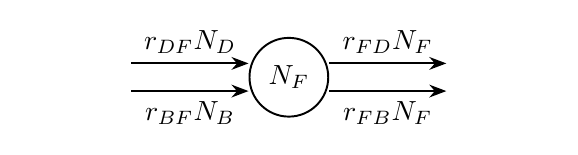
\begin{tikzpicture}[>=Stealth,->,line width=.7pt]
\matrix [matrix of math nodes,
column sep={3.2cm,between origins},
row sep={3.2cm,between origins},
nodes={circle, draw, minimum size=1cm}]
{
& |(1)| N_F & \\};
 
 \draw [transform canvas={xshift=0pt,yshift=-5pt}] (1)--(2,0) node [midway, below] {$r_{FB}N_F$};
  \draw [transform canvas={xshift=0pt,yshift=5pt}] (1)--(2,0) node [midway, above] {$r_{FD}N_F$};
 
 
 \draw [transform canvas={xshift=0pt,yshift=-5pt}] (-2,0)--(1) node [midway, below] {$r_{BF}N_B$};
  \draw [transform canvas={xshift=0pt,yshift=5pt}] (-2,0)--(1) node [midway, above] {$r_{DF}N_D$};
 
\end{tikzpicture}
\end{document}
